
\documentclass[13pt,compress]{beamer}
% deactivate beamer navigation
%\setbeamertemplate{navigation symbols}{}
%\usepackage{geometry}
%\geometry{papersize={180mm, 135mm}, top={1-last}, trim=0mm 0mm 45mm 0mm1.5mm} % 210mm, 297mm

\usepackage[nospeakermargin]{../style/lmu-lecture}

\setbeamertemplate{frametitle}{\expandafter\uppercase\expandafter\insertframetitle}
%\useoutertheme{metropolis}
% remove section slides
\AtBeginSection[]
{
  \begin{frame}<beamer>
    \frametitle{Part 1}
    \tableofcontents[currentsection]
  \end{frame}
}
% includepdf slides, pagecommad will set counter for framenumber
\usepackage{pdfpages}
\includepdfset{trim=0mm 0mm 0mm 0mm, pagecommand={\global\setcounter{framenumber}{\value{page}}}}
% trim=0mm 6mm 0mm 0mm, offset=0 15,
% add footer:
\usepackage{framed, color}
\usepackage{xcolor}
%\iffalse
% \setbeamertemplate{footline}[text line]{%
%     \noindent\hspace*{\dimexpr-\oddsidemargin-1in\relax}%
%      \colorbox{white}{
%      \makebox[\dimexpr\paperwidth-2\fboxsep\relax]{
%      \color{black}
%      \begin{minipage}[c][4.5ex][c]{0.5\linewidth}
%        \secname
%      \end{minipage}
%      \hfill\begin{minipage}[c][4.5ex][c]{0.5\linewidth}
%        \flushright
%        \insertframenumber{}~/~\inserttotalframenumber~~
%      \end{minipage}
%      }}%
%   \hspace*{-\paperwidth}
% }



% \setbeamertemplate{footline}[text line]{%
%     \noindent\hspace*{\dimexpr-\oddsidemargin-1in\relax}%
%      \colorbox{white}{
%      \makebox[\dimexpr\paperwidth-9ex\relax]{
%      \color{black}
%      \begin{minipage}[c][2.5ex][b]{0.5\linewidth}
%        \secname
%      \end{minipage}
%      \hfill\begin{minipage}[c][2.5ex][b]{0.5\linewidth}
%        \flushright
%        %\insertframenumber{}~/~\inserttotalframenumber~~
%      \end{minipage}
%      }}%
%      \begin{minipage}[c][3.5ex][t]{6.5ex}
%        \flushright
%        \fontsize{4pt}{6}\selectfont\transparent{0.3}\insertframenumber{}~/~\inserttotalframenumber~~
%      \end{minipage}
%   \hspace*{-\paperwidth}
% }
%\fi

\title{Introduction to Machine Learning\\with R and mlr3}
\author{Bernd Bischl \& Marvin N. Wright}
%\institute{Essential Data Science Training}
\date{DAGStat, March 2025}

\begin{document}
\setbeamercolor{background canvas}{bg=}

% General remark: hyperlinks in included pdfs are not clickable anymore in the combined pdf

\frame{\titlepage}

\subsection{Regularization: Introduction}
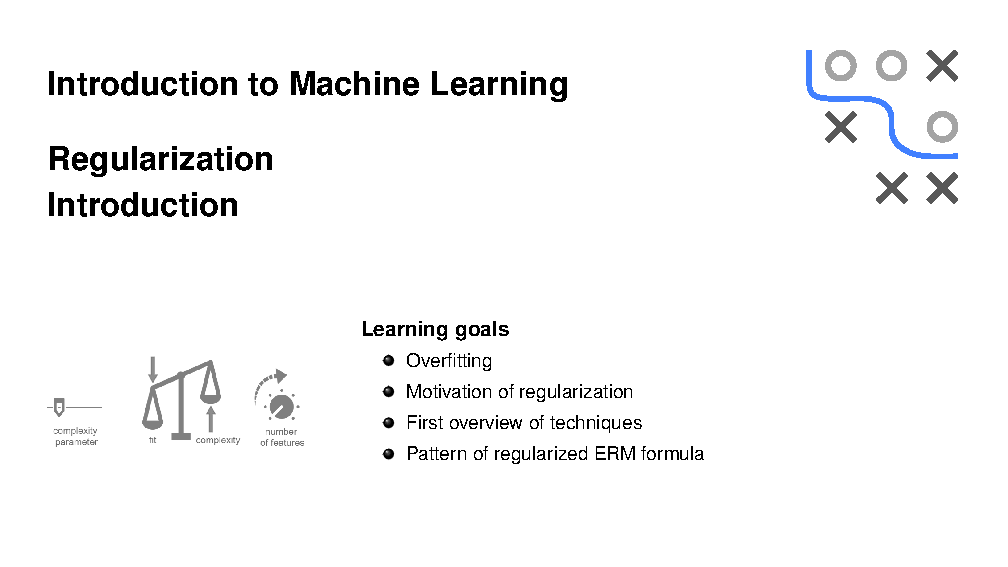
\includepdf[pages=-, trim=0mm 0mm 45mm 0mm]{../slds-lecture-pdfs/lecture_sl/slides-pdf/slides-regu-intro.pdf}

\subsection{Regularization: Ridge Regression}
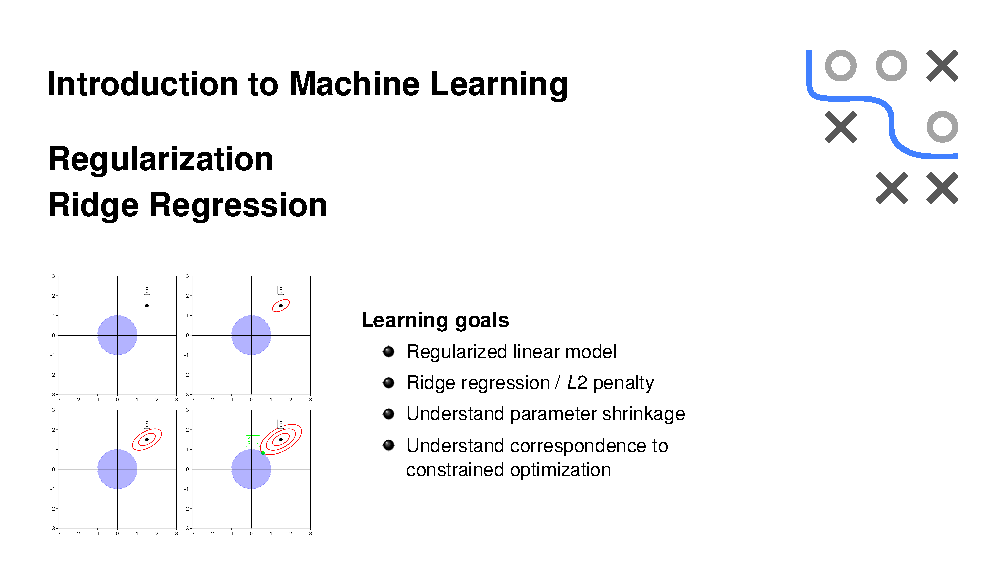
\includepdf[pages=-, trim=0mm 0mm 45mm 0mm]{../slds-lecture-pdfs/lecture_sl/slides-pdf/slides-regu-l2.pdf}

\subsection{Regularization: Lasso Regression}
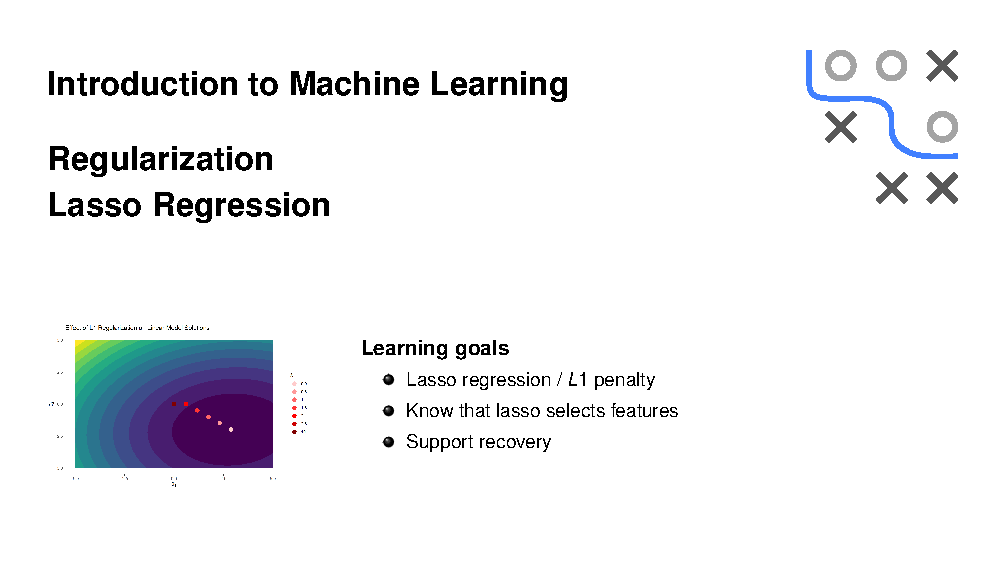
\includepdf[pages=-, trim=0mm 0mm 45mm 0mm]{../slds-lecture-pdfs/lecture_sl/slides-pdf/slides-regu-l1.pdf}

\subsection{Regularization: Lasso vs. Ridge}
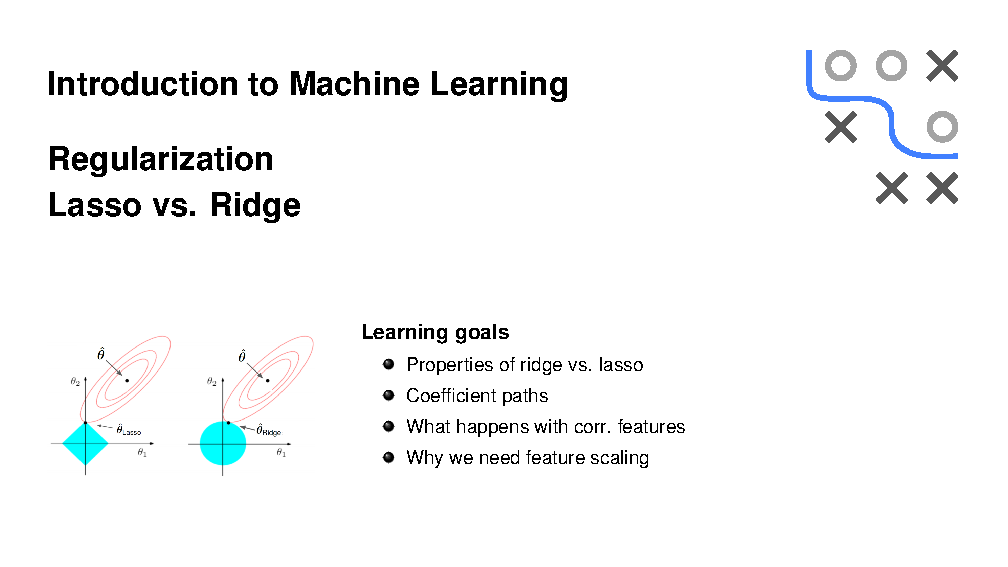
\includepdf[pages=-, trim=0mm 0mm 45mm 0mm]{../slds-lecture-pdfs/lecture_sl/slides-pdf/slides-regu-l1vsl2.pdf}

\subsection{Regularization: Elastic Net and GLMs}
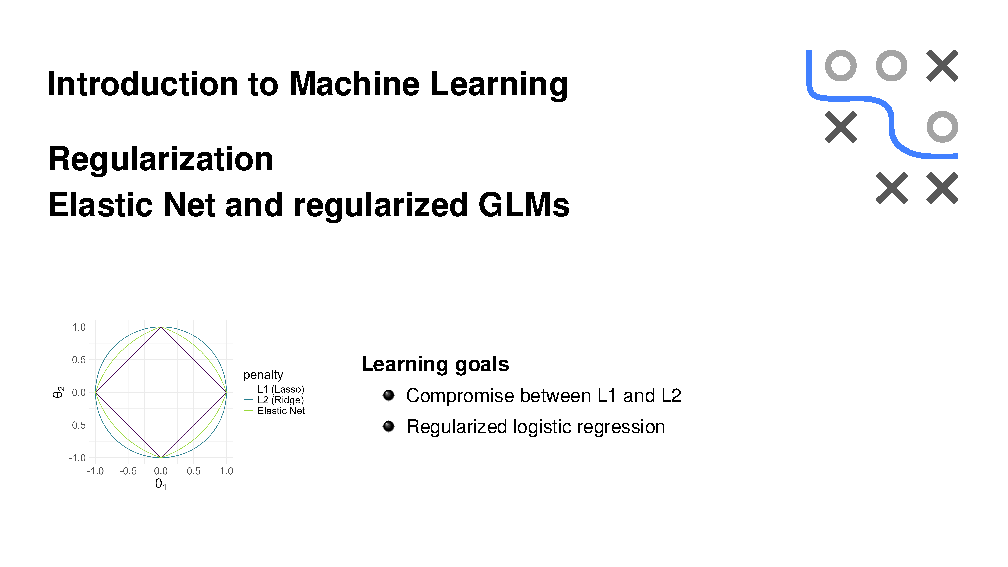
\includepdf[pages=-, trim=0mm 0mm 45mm 0mm]{../slds-lecture-pdfs/lecture_sl/slides-pdf/slides-regu-enetlogreg.pdf}

%\subsection{Regularization for Underdetermined Problem}
%\includepdf[pages=-, trim=0mm 0mm 45mm 0mm]{../slds-lecture-pdfs/lecture_sl/slides-pdf/slides-regu-underdetermined.pdf}

\subsection{Regularization: Other Types}
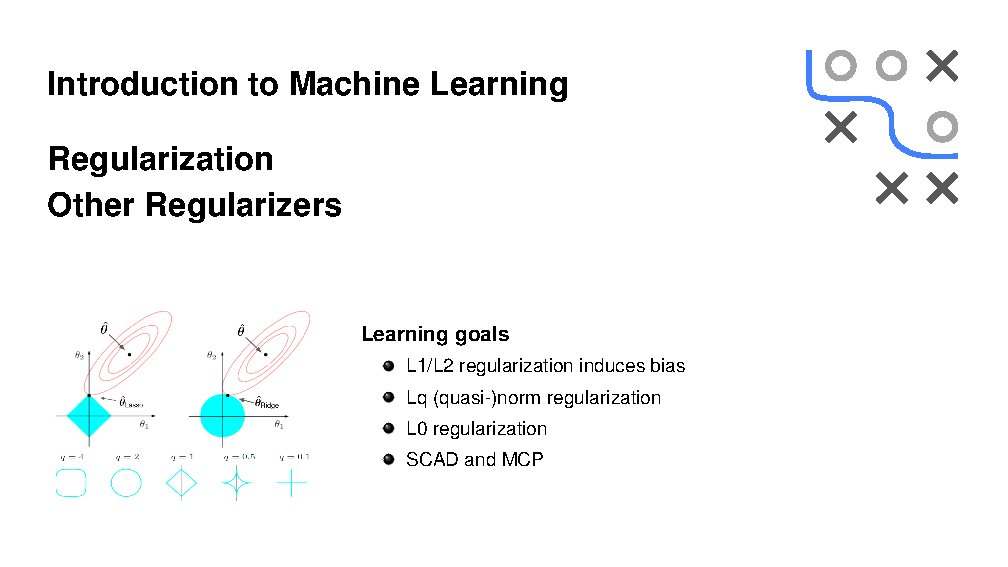
\includepdf[pages=-, trim=0mm 0mm 45mm 0mm]{../slds-lecture-pdfs/lecture_sl/slides-pdf/slides-regu-others.pdf}

%%%%%%%%%%%%%%%%%%%%%

\subsection{Regularization: Non-Linear Models and Structural Risk Minimization}
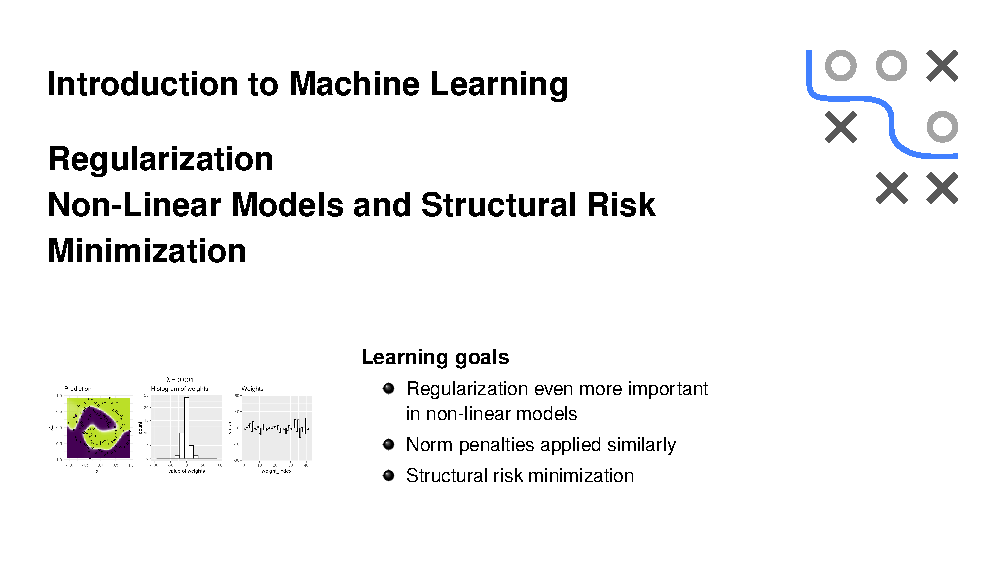
\includepdf[pages=-, trim=0mm 0mm 45mm 0mm]{../slds-lecture-pdfs/lecture_sl/slides-pdf/slides-regu-nonlin.pdf}

\subsection{Regularization: Bayesian Priors}
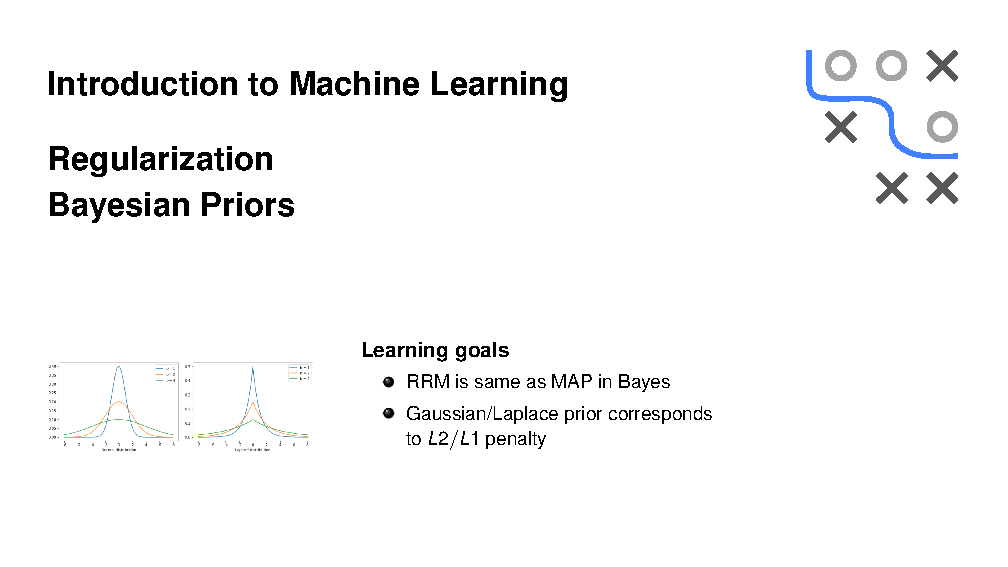
\includepdf[pages=-, trim=0mm 0mm 45mm 0mm]{../slds-lecture-pdfs/lecture_sl/slides-pdf/slides-regu-bayes.pdf}

\subsection{Regularization: Weight Decay and L2}
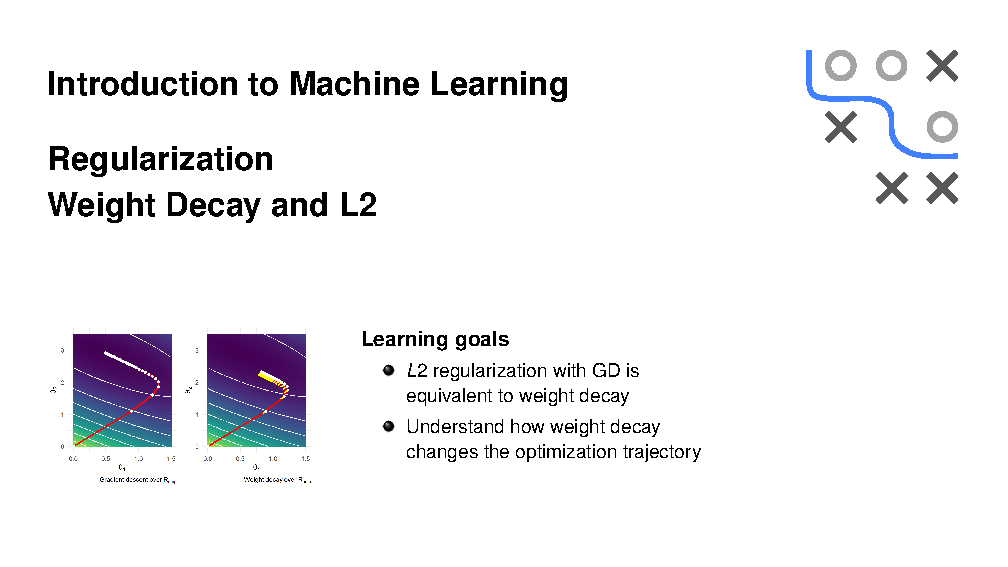
\includepdf[pages=-, trim=0mm 0mm 45mm 0mm]{../slds-lecture-pdfs/lecture_sl/slides-pdf/slides-regu-wd-vs-l2.pdf}

\subsection{Regularization: Geometric Analysis of L2}
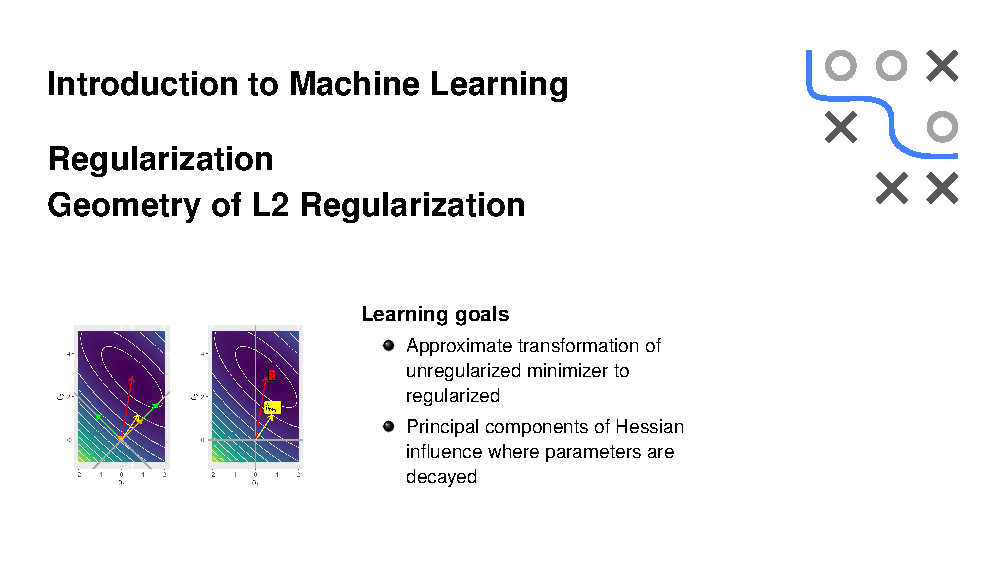
\includepdf[pages=-, trim=0mm 0mm 45mm 0mm]{../slds-lecture-pdfs/lecture_sl/slides-pdf/slides-regu-geom-l2.pdf}

\subsection{Regularization: Geometric Analysis of L1}
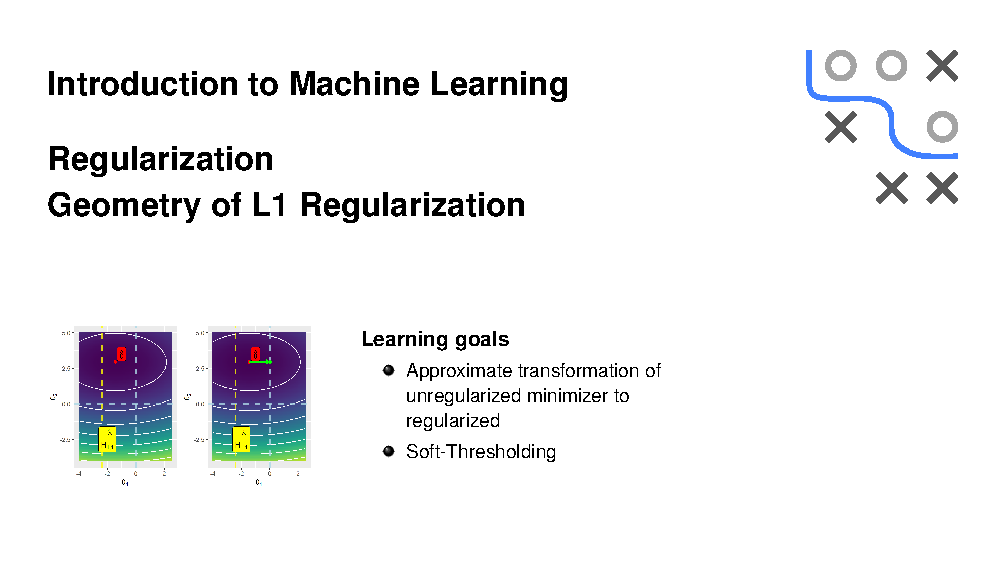
\includepdf[pages=-, trim=0mm 0mm 45mm 0mm]{../slds-lecture-pdfs/lecture_sl/slides-pdf/slides-regu-geom-l1.pdf}

\subsection{Regularization: Early Stopping}
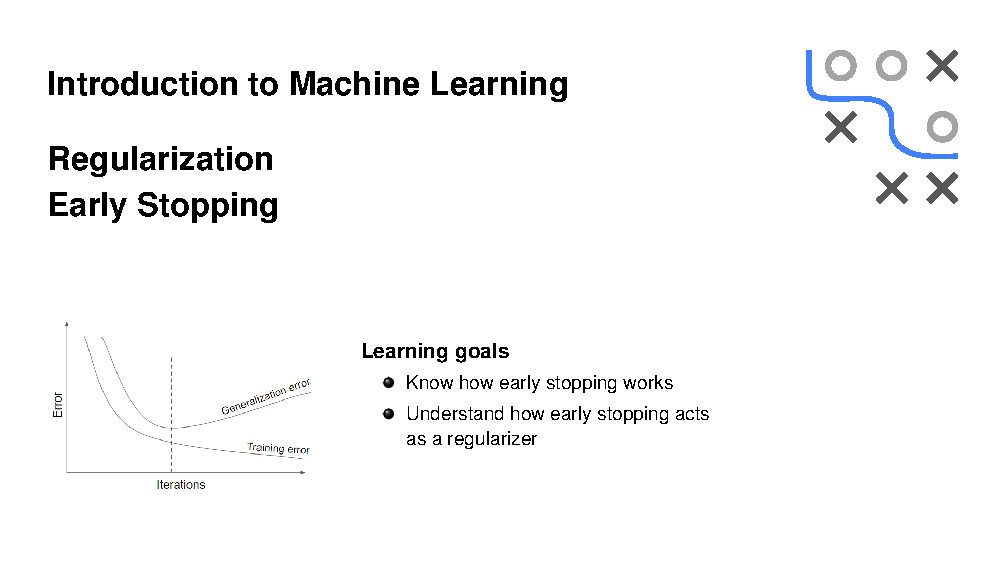
\includepdf[pages=-, trim=0mm 0mm 45mm 0mm]{../slds-lecture-pdfs/lecture_sl/slides-pdf/slides-regu-early-stopping.pdf}

\subsection{Regularization: Perspectives on Ridge Regression (Deep-Dive)}
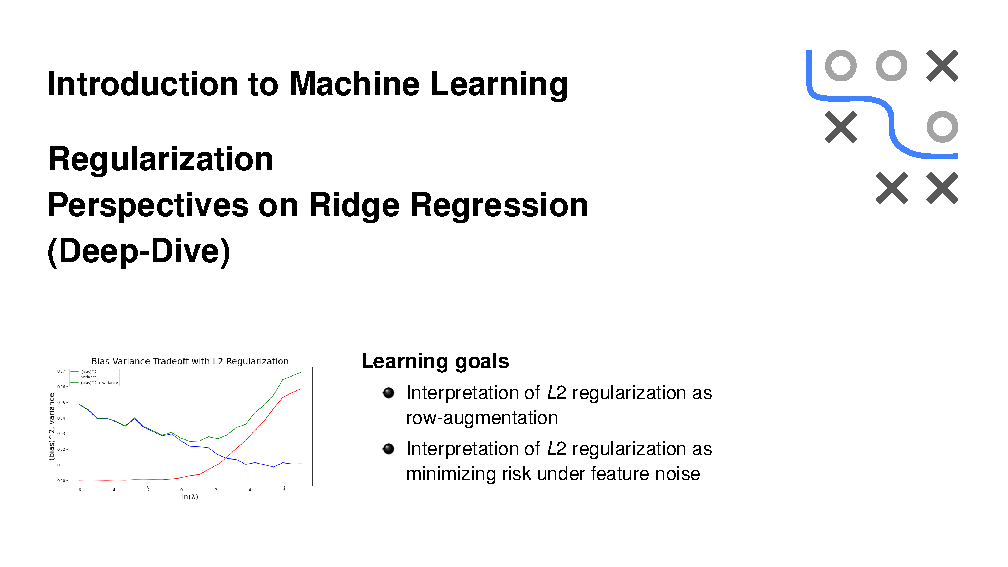
\includepdf[pages=-, trim=0mm 0mm 45mm 0mm]{../slds-lecture-pdfs/lecture_sl/slides-pdf/slides-regu-ridge-deepdive.pdf}

\subsection{Regularization: Soft-thresholding and L1 regularization (Deep-Dive)}
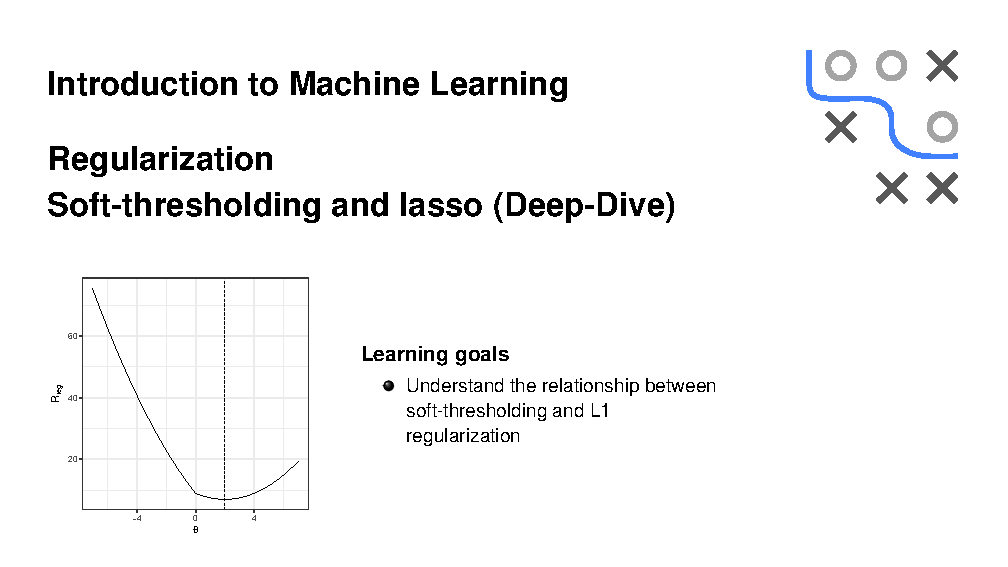
\includepdf[pages=-, trim=0mm 0mm 45mm 0mm]{../slds-lecture-pdfs/lecture_sl/slides-pdf/slides-regu-lasso-deepdive.pdf}




\subsection{Introduction}
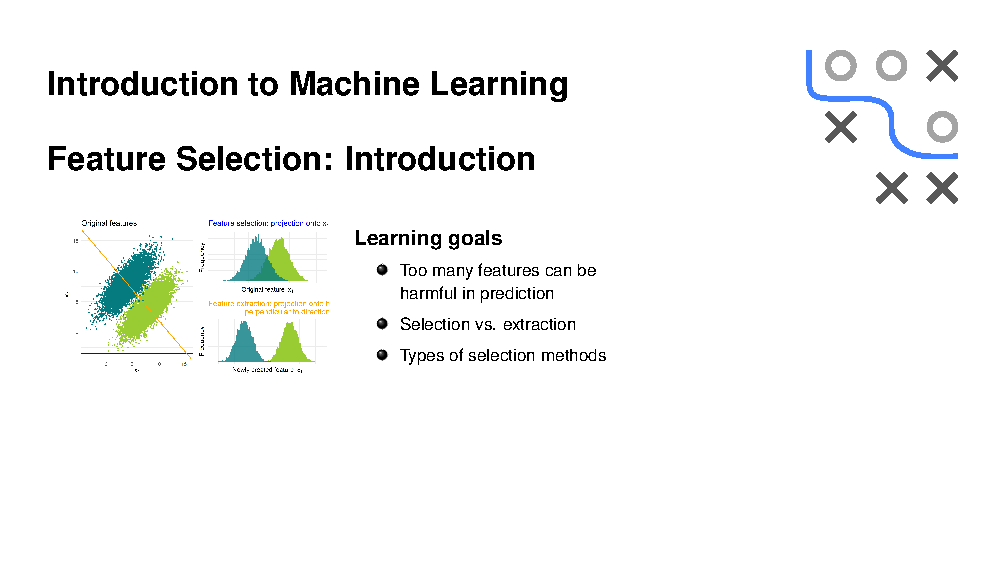
\includepdf[pages=-, trim=0mm 0mm 45mm 0mm]{../slds-lecture-pdfs/lecture_sl/slides-fs-introduction.pdf}

\subsection{Motivating examples}
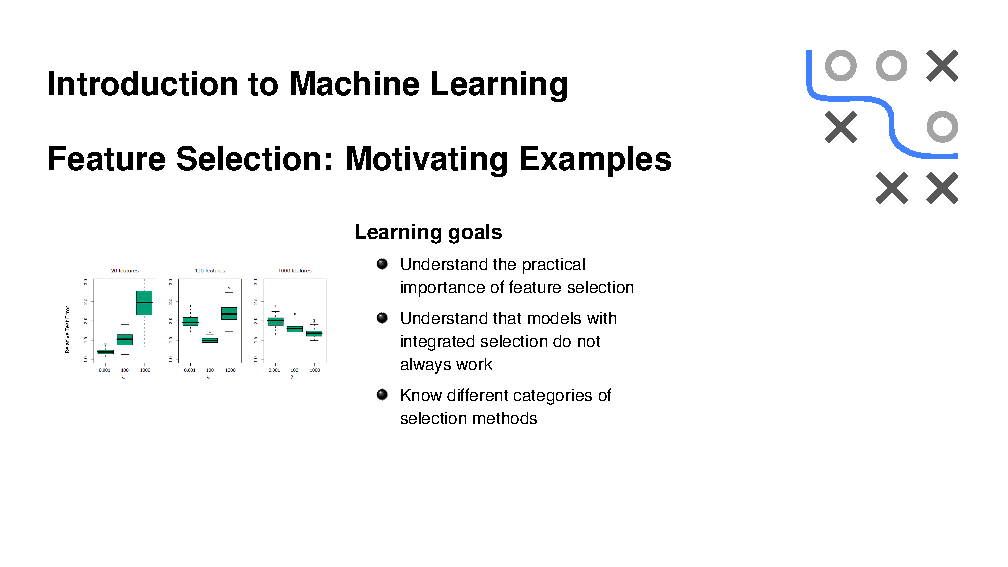
\includepdf[pages=-, trim=0mm 0mm 45mm 0mm]{../slds-lecture-pdfs/lecture_sl/slides-fs-motivating-examples.pdf}

\subsection{Filter Methods}
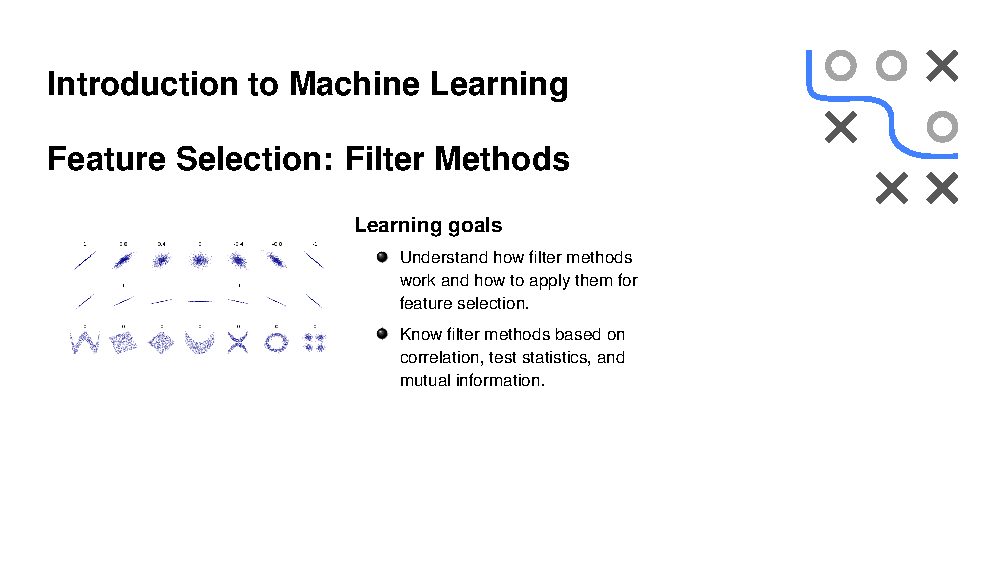
\includepdf[pages=-, trim=0mm 0mm 45mm 0mm]{../slds-lecture-pdfs/lecture_sl/slides-fs-filters1.pdf}

\subsection{Filter Examples and Caveats}
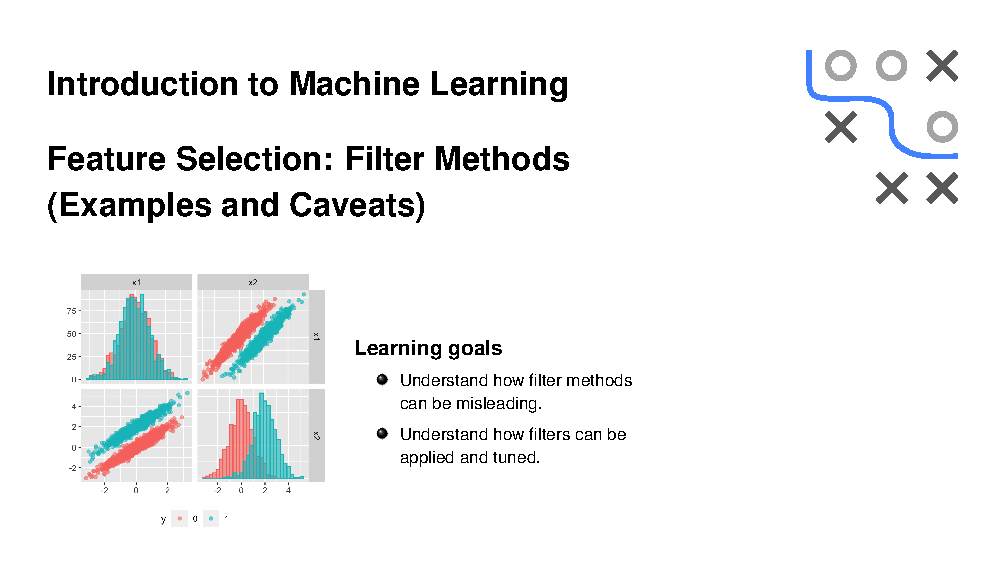
\includepdf[pages=-, trim=0mm 0mm 45mm 0mm]{../slds-lecture-pdfs/lecture_sl/slides-fs-filters2.pdf}

\subsection{Wrapper}
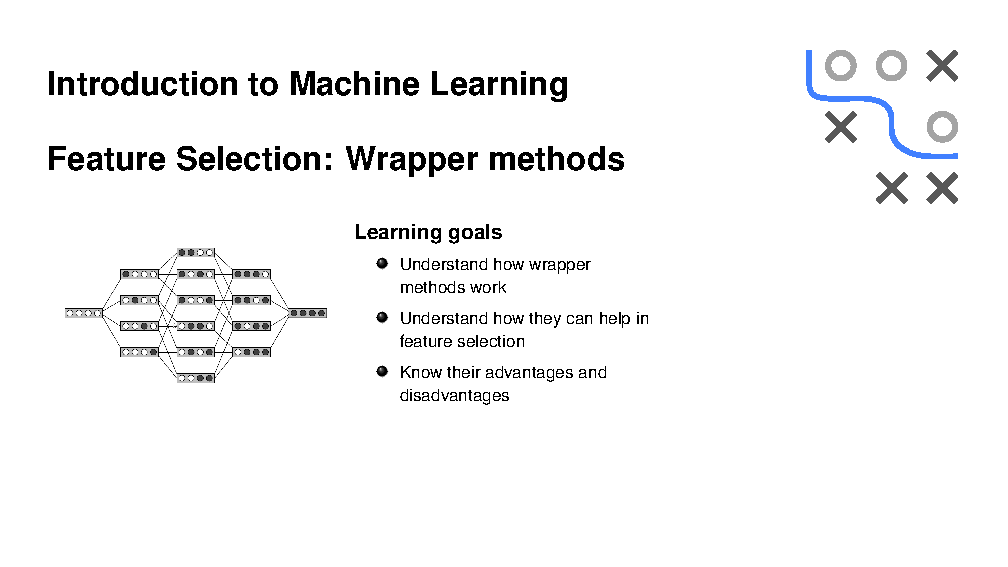
\includepdf[pages=-, trim=0mm 0mm 45mm 0mm]{../slds-lecture-pdfs/lecture_sl/slides-fs-wrapper.pdf}

\end{document}

